Besides the extension of the Script Assembler's capabilities and the creation of a new EBNF language that makes the software more extendable, another main focus of the project is the creation of a mockup of the TestRail database. This mockup is not only made for testing purposes, but allows the user to work independently of the TestRail instance. The mockup is designed to be as close to the real TestRail database as possible, allowing a seamless switch between the two instances. This means that all functionalities that are available in the real TestRail database are also available in the new mockup.

This section aims to give an overview of the different types of databases, the structure and functionalities of the TestRail database specifically, the resulting design and implementation of the mockup database, and the way the database switch is finally implemented.

\section{Types of Databases}

Depending on the requirements of a given project, different types of databases are suitable for different use cases. It is important to analyze what qualities are needed and which qualities are negligible to find the best fitting solution. 

The most important qualities of a database type can be expressed in the following categories:

\begin{itemize}
    \item \textbf{Data Model:} \\
    The data model of a certain database type describes how the data is structured and stored. This can be in the form of tables, documents, graphs or other structures. The data model has a notable impact on aspects like performance and scalability.

    \item \textbf{Storage Architecture:} \\
    The storage architecture of a database type not only describes how the data is stored, but also how it may be accessed, managed and distributed. This can be in the form of a single server, a cluster of servers or even a distributed network of servers across the globe.

    \item \textbf{Query Model:} \\
    The query model of a database type describes the means of accessing the data. This can occur in the form of a specifically designed query language, an API or other methods. This has an undeniable impact on the ease of use of the database and how the user writes and optimizes queries.
\end{itemize}

Based on these qualities, various databases types have been developed, each with their own unique advantages and disadvantages. Some of the most common types of databases include but are not limited to relational databases, object-oriented databases and NoSQL databases, which can be further categorized by the data model they use, such as document stores, key-value stores, column-family stores and graph databases \cite{DigitalOceanDatabaseTypes}.

\section{Relational Databases}

For the purpose of this project, we will take a closer look at relational databases, as this is the type of database that TestRail uses. 

\subsection{Structure of Relational Databases}

Relational databases are based on the relational model, which organizes its data into tables, consisting of rows and columns. Each table represents a specific entity and each row in the table represents an instance of that entity. The columns in the table represent the attributes of the entity. 

Relationships between these entities can be established through the use of keys. A primary key is a unique identifier for each instance of an entity, while a foreign key is a reference to the primary key of another entity. Meaningful relationships between entities can be built with the usage of these keys, allowing complex queries to be executed across multiple linked entities \cite{WikipediaRelationalDatabase}.

Grouping in queries allows for the aggregation of data based on specific attributes, while joins allow for the combination of data from multiple tables based on the established relationships.

\begin{figure}[ht]
    \centering
    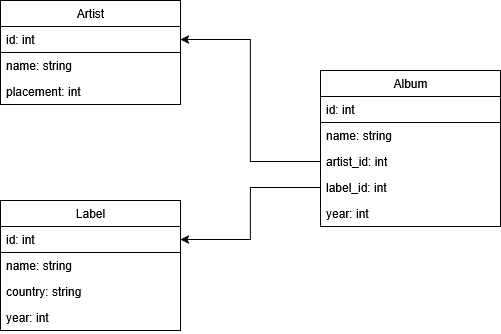
\includegraphics[width=0.8\textwidth]{pics/simple-erd.png}
    \caption{Simple Diagram showcasing the relationship between three entities in a relational database.}
    \label{fig:erd}
\end{figure}

In figure \ref{fig:erd}, we can see a simplified example of a relational database structure. The three entities "Artist", "Label" and "Album" are represented as tables, with their respective attributes as columns. The relationships between the entities are established through the usage of primary and foreign keys, allowing for queries to be executed across multiple linked entities. For example, we can query for all albums by a specific artist or a specific label.

\subsection{ACID}

ACID is an acronym that stands for the four key properties of a safe database transaction:

\begin{itemize}
    \item \textbf{Atomicity:} \\ 
    Atomicity ensures that a transaction, which is often a sequence of multiple operations, is treated as a single unit. This means that either all operations within a given transaction are executed successfully, or none of them are. If any operation of the transaction fails due to an error, a power outage or any other issue, the entire transaction is rolled back to its previous state before the transaction began. This guarantees that the database remains consistent and prevents data corruption or loss that could occur if only part of the transaction were to be executed.
    
    \item \textbf{Consistency:} \\
    Consistency ensures that the database can only be brought from one valid consistent state to another, while following all defined rules, constraints and triggers. Invalid transactions that violate any of the defined rules are rolled back accordingly, ensuring that the database remains consistent.
    
    \item \textbf{Isolation:} \\
    Isolation ensures that concurrent transactions have no impact on each other. This means that the effects of a transaction in progress are not visible to other transactions until it completes successfully. This prevents a number of issues that would otherwise arise from concurrent transactions, like dirty reads, where one transaction reads data that has been modified by another transaction but not yet fully committed, potentially leading to incorrect results.
    
    \item \textbf{Durability:} \\ 
    Durability ensures that once a transaction has been successfully completed and committed, the state of the database persists even in the case of a crash, power failure or any other issue. 
\end{itemize}

Databases that adhere to these properties are considered to be reliable and safe for use in critical environments, as they guarantee that the data not only remains consistent, but also that it is not lost or corrupted due to unforseen events \cite{WikipediaACID}.

\subsection{Advantages and Disadvantages of Relational Databases}

One of the main strengths of relational databases is their ability to handle long and complex queries across multiple linked entities with the usage of foreign keys and joins. The consistency and integrity of the data is guaranteed by the ACID properties. On top of that, relational databases are some of the most widely used and well-known types of databases, which means that there are a lot of resources and a large community available for support and development. 

However, relational databases can struggle with scalability and performance when dealing with large volumes of data or high traffic. The fixed schema of relational databases can also be a disadvantage, as it can make it difficult to adapt to changing requirements or to handle unstructured data. Additionally, the execution of complex queries can lead to performance issues on larger datasets.

\section{The TestRail Database}

TestRail is a web-based test management tool that provides a wide range of features for managing and organizing test cases, test runs and test results. The relational database in the background of TestRail is used to store all of the data related to these features. The user can interact with the database directly by using the TestRail API, although the database itself is not directly accessible to the user. 

Thus, for the creation of the mockup database, the structure and functionalities of the TestRail database have to be studied and analyzed based on the API documentation and the structure of its response data. While the mockup database doesn't have to be an exact replica of the TestRail database, the functionalities used by the Script Assembler need to deliver responses with identical structure to ensure the switch between databases can occur without any issues.

In order to achieve this, the most important entities and their relationships have to be identified.

\subsection{Test Cases}

Test cases can be seen as the most fundamental entity in the TestRail system, as they represent the individual tests that are to be executed. Test cases have a number of attributes, such as a title, description, type and the test steps that need to be executed. Test cases are furthermore linked to test suites and sections. 

\subsection{Projects, Suites and Sections}

Projects are the highest level of organization in TestRail, representing a specific testing effort or initiative. Each project can contain multiple test suites, which are collections of test cases. The test cases of Suites can further be organized into sections, allowing for more specific grouping and categorization. These relationships are an essential part of the database structure that needs to be replicated.

\subsection{Test Runs}

A test run represents a specific execution of test cases. Test runs are linked to test cases and contain information about the execution, such as the status of each case, the tester who executed the run and any relevant comments or other metadata. Test runs make the tracking and management of test executions possible. Importantly, a test run can only be created for test cases that are contained in one singular test suite.

\subsection{Test Plans}

Test plans are used to organize and manage test runs. TestRail allows the user to group multiple test runs into a test plan, which alleviates the need to manage each run individually.

\subsection{Test Results}

Test results represent the outcome of a test case within a test run. Test results mainly consist of a status, which can contain, but is not limited to:

\begin{itemize}
    \item \textbf{Passed} \\
    A test case is marked as passed when it has been successfully executed and all results are as expected.

    \item \textbf{Failed} \\
    A test case is marked as failed when it has been executed but the results are not as expected, meaning that the tested functionality does not work as intended.

    \item \textbf{Untested} \\
    A test case that hasn't been assigned a status yet is marked as untested.

    \item \textbf{Retest} \\
    A test case is marked as retest when it has failed previously, but has been fixed and is now ready to be tested again.

    \item \textbf{Blocked} \\
    A test case is marked as blocked when it cannot be executed due to an error that is not related to the functionality being tested.
\end{itemize}

\subsection{Users}

Users represent the individuals who interact with the TestRail system. Users can have different roles and permissions within the system. They can be assigned to test runs, test plans or other entities as creators. With the user entity it is possible to track who is responsible for which run and plan.

\section{PostgreSQL}

For the implementation of the mockup database, PostgreSQL was chosen as the database management system, as it is an open-source database that is not only widely used but also well-known for its reliability and performance. 

PostgreSQL is not only a database management system that the team is familiar with, but it also provides all the necessary features and capabilites needed for the implementation of this part of the project. It supports the relational data model, which is needed for replacing the TestRail database, and it guarantees the reliability and consistency of its data with the ACID properties.

\subsection{pgAdmin}

The open-source management tool "pgAdmin" is used for the administration of the PostgreSQL database, as it provides an easily navigable user interface for management, query execution and other administrative tasks.

\begin{figure}[ht]
    \centering
    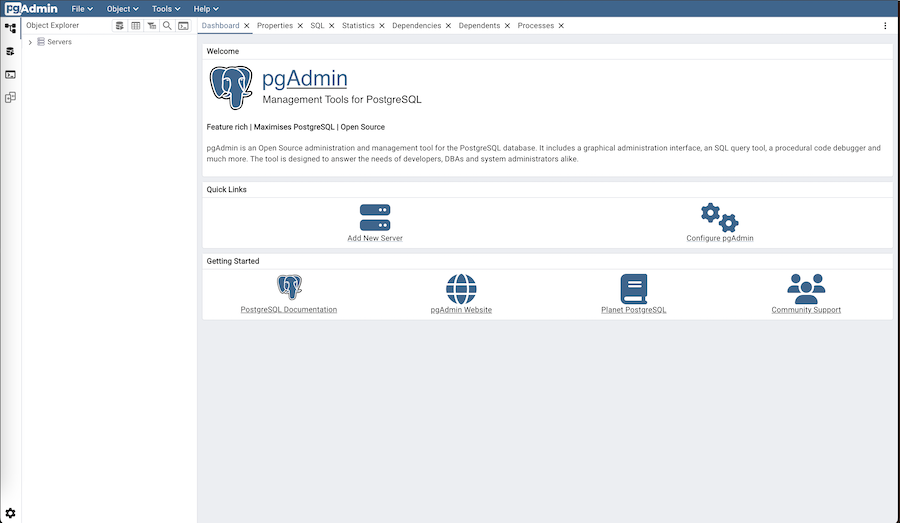
\includegraphics[width=0.95\textwidth]{pics/pgadmin-interface.png}
    \caption{Screenshot of the pgAdmin interface \cite{pgAdminInterface}.}
    \label{fig:pgadmin-interface}
\end{figure}

The current version of pgAdmin, which is pgAdmin 4, provides a wide range of features for managing and administering PostgreSQL databases, some of which include but are not limited to the following: \cite{pgAdminInterface}.

\begin{itemize}
    \item \textbf{SQL query tool:} \\
    Inside pgAdmin, there is a built-in SQL editor that allows users to write and execute SQL queries directly against the database. This tool provides syntax highlighting, further aiding the user in writing correct queries.

    \item \textbf{Direct data editing:} \\
    The tables in a database can be directly edited through the interface, allowing for quick and easy modifications of single points of data without the need to write and execute SQL queries. Caution should be taken when using this feature however, as the quick and easy nature of this feature can lead to unintended consequences.

    \item \textbf{Management of multiple databases:} \\
    The pgAdmin interface allows the management of multiple databases within the same interface, allowing for intuitive switching between independent databases. 
\end{itemize}

\section{First Approaches}

Early into the development of the database, two main approaches were considered for how the database should interact with the backend of the main system. 

One approach was to create an API that would allow the main system to interact with the database through API calls. This would have resulted in a clear separation between the database and the main system.

The other approach was to work in the preexisting backend to connect to the database directly. This approach was ultimately chosen, as it not only makes the switch between the two databases simpler, but also integrates the functionality of the new database directly into the main system. This approach was further endorsed by the supervisor of the project, as it helps the system to eventually transition away from the TestRail database and towards the new mockup database, which allows for more independence and expandability in the future.

The python library "psycopg" is used for the connection between the main system and the PostgreSQL database. This library provides a simple and efficient way to connect to the PostgreSQL database and execute various commands and queries. It also provides support for connection pooling, which can help to improve the performance of the database interactions.

\section{Database Connections in the System}

The following section aims to give a brief look into the structure and functionalities of not only the existing TestRail database connection, but also the new PostgreSQL mockup database. The goal is to show how the new database is designed to replicate the implementations of the TestRail connection, while also highlighting clear differences on a technical level.

\subsection{Existing TestRail Functionality}

The existing funtionalities concerning the TestRail connection is contained within the TRSession class, which is responsible for all interactions with the database. This class contains functions for retrieving and creating test cases, runs, plans and results, as well as other relevant data. 

The communication with the TestRail database is achieved through the usage of the TestRail API, which provides all necessary reading and writing functionalities.

\begin{lstlisting}[caption={Code snippet of the get\_case\_title function within the TRSession class.}, label={lst:tr-function}]

    def get_case_title(self, case_id: int, safe_name: bool = False) -> str | None:
        response = self.do_request(f"get_case/{case_id}", TRConst.REQUEST_TYPE_GET)
        if not response:
            return None
        if len(response) <= 0:
            self.log.warning(f"could not find a result for test case: {case_id}")
            return None
        if not safe_name:
            return response['title']
        return response['title'].replace(":", "")

\end{lstlisting}

In listing \ref{lst:tr-function}, one of the functions of the TRSession class can be seen. This function is responsible for retrieving the title of a test case based on its ID. Using the ID of the wanted test case, a GET request is sent to the TestRail API, which then returns the relevant data. The function then processes the response data and returns the title. 

All functions of the TRSession class follow a similar structure, with the type of interaction with the API being the main difference. For example, functions that create new entities in the database use POST requests and send the relevant data in the body of the request.

\subsection{DBSession}

The DBSession class is designed to replicate all used functionalities of the exisitng TRSession class, while replacing the communication with the TestRail API with a direct connection to the PostgreSQL database, using the "psycopg" python library. It is strictly necessary that the functions of the DBSession have the same name, parameters and return values as the functions of the TRSession class, in order to avoid major conflicts when switching between the two database connections.

\begin{lstlisting}[caption={Code snippet of the get\_case\_title function within the DBSession class.}, label={lst:db-function}]

    def get_case_title(self, case_id: int, safe_name: bool = False) -> str | None:

        if case_id == None:
            print("Did not get a case_id")
            return None
        
        if case_id < 0:
            print(f"Invalid value for case_id: {case_id}")
            return None
        
        self.cursor.execute("SELECT title FROM test_cases WHERE id = %s", (case_id,))

        result = self.cursor.fetchone()

        if result != None:
            return str(result[0])
        
        return None

\end{lstlisting}

In listing \ref{lst:db-function}, the same function as in listing \ref{lst:tr-function} can be seen, but this time within the DBSession class. Thus, while the parameters and return value of the function are identical to the one in the TRSession class, the implementation is different.

Instead of interacting with an API, this function uses a connection to the PostgreSQL database to execute a SQL query that retrieves the title of the specified test case. 

\section{Integration of the DBSession Class}

Since the DBSession class replicates all essential functions of the TRSession class, the switch between database usages can be achieved easily.

Any occurrence of the TRSession class within the backend of the system is now denoted as a TRSession or DBSession, using a pipe symbol. This means that at system startup, the appropriate session class has to be identified and initialized accordingly. 

\begin{lstlisting}[caption={Code snippet showcasing a function that takes a parameter that can be either a TRSession or a DBSession.}, label={lst:tr-or-db}]

    def fetch_cases(self, testrail: TRSession | DBSession):
        # Function implementation

\end{lstlisting}

This way, the TRSession functionalities remain unaltered, while the possibility of using the DBSession is a new feature that can be easily switched on or off.

\subsection{Switching Between Databases}

The switch between the two databases is implemented in a way that allows the user to easily and definitively choose which database should be used at the execution of the python script. This is achieved by using a command line argument that can be passed when executing the script. The argument is then processed and the appropriate database instance is initialized based on if the argument is present or not. 

\begin{verbatim}
    python ./broker.py
\end{verbatim}

Here, the standard TestRail database is used, as no argument is passed to the script.

\begin{verbatim}
    python ./broker.py -db
    # OR
    python ./broker.py --database
\end{verbatim}

Here, the PostgreSQL mockup database is used, as the argument is passed to the script. The argument can either be a short version, or a long version, as both are processed in the same way and lead to the same result.

\section{The PostgreSQL Database}

Since the structure of the TestRail database is not publicly available, the structure of the PostgreSQL mockup database is based on the structure of the response data the TestRail API provides. All entities contain their respective attributes, as well as keys that establish the relationships between the different entities.

It is important to note that the relationships between entities are not made with the usage of foreign keys, as the logic for the relationships is implemented in the backend of the system, and the database is only used for storing data. While this is not the most efficient way to implement the relationships between entities, as a mockup database, it is sufficient for the purpose of this project. Despite that, in section \ref{sec:potential-future-steps}, potential future steps are discussed, one of which is the implementation of proper relationships between entities with the usage of foreign keys.

The database contains tables for all the entities of the TestRail system, that are relevant for the functionalities of the Script Assembler. All entities are listed below, along with their respective attributes.

Every entity contains an \textit{id} attribute, signifying the unique identifies for each instance of the entity, with the datatype of \textit{serial}, which means that the integer value of the attribute is automatically incremented with each new instance of the entity. Since this attribute is present in all entities, it will not be listed for each entity separately.

\subsection{Case Types}

Case Types are used to categorize the test cases based on their type, such as functional, performance or security test cases. This is mainly used to group test cases together and strictly serve the organizational purposes of the system.

This table has the following attributes:
\begin{itemize}
    \item \textbf{is_default:} \\
    This attribute is a boolean value that is set to true for one specific case type, which is assigned as the default case type. All other case types have this attribute set to false.

    \item \textbf{case_name:} \\
    This attribute is a string value that contains the name of the case type.
\end{itemize}

\subsection{Groups}

Groups are used to categorize users based on their roles, permissions or tasks. Similarily to case types, groups are mainly used for organizational purposes.

This table has the following attributes:
\begin{itemize}
    \item \textbf{name:} \\
    This attribute is a string value that contains the name of the group.

    \item \textbf{user_ids:} \\
    This attribute is an array of integers that contains the IDs of all users assigned to the specific group.
\end{itemize}

\subsection{Priorities}

Priorities are used to order test cases in the system. Test cases with a higher value of priority are considered more important and are therefore executed before others with a lower value of priority. This also influences the ordering of test cases in the user interface, as well as the order they are assembled in the final script.

This table has the following attributes:
\begin{itemize}
    \item \textbf{is_default:} \\
    This attribute is a boolean value that is set to true for one specific priority, which is assigned as the default priority. All other priorities have this attribute set to false.

    \item \textbf{prio_name:} \\
    This attribute is a string value that contains the name of the priority.

    \item \textbf{priority:} \\
    This attribute is an integer value that contains the priority level, with higher values corresponding to a higher priority.

    \item \textbf{short_name:} \\
    This attribute is a string value that contains a short name alternative for the priority.
\end{itemize}

\subsection{Projects}

Projects are the uppermost level of organization in the system. They contain other entities such as test suites and by extension sections and test cases. Projects represent a specific testing effort or testing environment for an entire system.

This table has the following attributes:
\begin{itemize}
    \item \textbf{announcement:} \\
    This attribute is a string value that contains the announcement message for the project, which provides more information about the project and its purpose.

    \item \textbf{default_role_id:} \\
    This attribute is an integer value pointing to the ID of the role that is assigned as the default role for the project. This role is automatically assigned to all users that are added to the project, unless they are assigned a different role.

    \item \textbf{default_role:} \\
    This attribute is a string value that contains the name of the default role.

    \item \textbf{is_completed:} \\
    This attribute is a boolean value that indicates whether the project has been completed or not.

    \item \textbf{project_name:} \\
    This attribute is a string value that contains the name of the project.

    \item \textbf{show_announcement:} \\
    This attribute is a boolean value that indicates whether the announcement message of the project should be shown to users or not.

    \item \textbf{url:} \\
    This attribute is a string value that contains the URL of the project.

    \item \textbf{users:} \\
    This attribute is an array of integers that contains the IDs of all users assigned to the project.

    \item \textbf{completed_on:} \\
    This attribute is an integer value that contains the UNIX timestamp of when the project was completed.
\end{itemize}

\subsection{Test Suites}

Test Suites are collections of test cases that are grouped together based on their purpose or functionality.

This table has the following attributes:
\begin{itemize}
    \item \textbf{description:} \\
    This attribute is a string value that contains the description of the specific test suite.

    \item \textbf{name:} \\
    This attribute is a string value that contains the name of the test suite.

    \item \textbf{project_id:} \\
    This attribute is an integer value that contains the ID of the project that the test suite is assigned to.

    \item \textbf{url:} \\
    This attribute is a string value that contains the URL of the test suite.
\end{itemize}

\subsection{Sections}

Sections further divide and organize the test cases within a test suite.

This table has the following attributes:
\begin{itemize}
    \item \textbf{depth:} \\
    The depth attribute is an integer value that indicates the level of the section within the hierarchy of sections. The lower the value, the higher the section is in the hierarchy.

    \item \textbf{description:} \\
    This attribute is a string value that contains the description of the specific section.

    \item \textbf{display_name:} \\
    This attribute is a string value that contains a name of the section as it should be displayed in the user interface.

    \item \textbf{name:} \\
    This attribute is a string value that contains the name of the section.

    \item \textbf{parent_id:} \\
    Sections can be nested within other sections, which can be achieved by assigning a section as the parent of another. This attribute is an integer value that contains the ID of the parent section, if there is one. If this section is in the uppermost level of the hierarchy, it does not have a parent and therefore this attribute is set to null.

    \item \textbf{suite_id:} \\
    This attribute is an integer value that contains the ID of the test suite that the section is assigned to.
\end{itemize}

\subsection{Test Cases}

This table has the following attributes:
\begin{itemize}
    \item \textbf{} \\
\end{itemize}

\subsection{Test Results}

This table has the following attributes:
\begin{itemize}
    \item \textbf{} \\
\end{itemize}

\subsection{Test Runs}

This table has the following attributes:
\begin{itemize}
    \item \textbf{} \\
\end{itemize}

\subsection{Tests}

This table has the following attributes:
\begin{itemize}
    \item \textbf{} \\
\end{itemize}

\subsection{Users}

This table has the following attributes:
\begin{itemize}
    \item \textbf{} \\
\end{itemize}

\section{Potential Future Steps} \label{sec:potential-future-steps}

\subsection{Easier Creation of Test Cases}

TestRail provides a functionality for the creation of test cases through the API, as well as through their user interface. This makes the creation of new test cases in the database an easy task, especially with the user interface, as the user can efficiently create new test cases and other entities without having to worry about the structure of the database itself.

Currently, the creation of test cases in the PostgreSQL database is done manually by either executing SQL queries manually or by making use of the pgAdmin user interface. This is not only time-consuming, but also prone to errors, as the user has to ensure that all necessary attributes of the test case are filled in correctly and that the relationships between entities are established properly.

A potential future step to fix this issue would be to create a user interface that allows for the easier creation of test cases and other entities in the database. This system could either be a separate application that interacts with the database on its own, or it could be integrated into the existing system. 

\subsection{Information Security}

For convenience and ease of use, the users of the PostgreSQL database currently have their credentials stored in plain text within their respective columns in the database. While this is not an issue for the mockup database, as it is only used for testing purposes, if the PostgreSQL database approach is to be used in the future as a replacement for the TestRail database, it would be necessary to implement a system for encrypting or hashing the credentials of all users, in order to ensure the security of the database and the data it contains. 

This could be achieved by using a hashing algorithm to hash the passwords before storing them in the database, and then comparing the hashed password with the stored hash when a user attempts to log in. This would ensure that actual passwords cannot be retrieved from the database, even if the database is compromised.

Hasing is an irreversible process, meaning that once a password is hashed, it cannot be converted back to its plain text form. Encryption, on the other hand, is a reversible process, so it would be possible to retrieve the original password from the encrypted form if the key is known. While hashing is more secure for storing passwords, both methods are viable options for ensuring the security of credentials in the database.

\subsection{Implementation of Proper Relationships}

The relationships between entities in the PostgreSQL database are not implemented with the usage of foreign keys, but rather with the usage of keys that are processed in the backend of the system. The logic for the relationships is implemented in the backend, which means that the database is only used for strictly storing data. 

This is not the most efficient way to implement relationships, as it can lead to issues with data integrity, as well as performance issues when executing queries that involve multiple linked tables.

The logical next step to improve the implementation of the database would be to implement proper relationships between entities with the correct usage of foreign keys. 